\documentclass{beamer}
\usepackage{hyperref}
\usepackage[T1]{fontenc}
\usepackage{latexsym,amsmath,xcolor,multicol,booktabs,calligra}
\usepackage{graphicx,listings,stackengine}

\author{Shengbo Tong}
\title{ZhuLong}
\subtitle{An Execution-Grounded Self-Evolving Agent for EDA Scripting}
\institute{Tsinghua University, CXMT}
\date{2026.8.7}
\usepackage{Tsinghua}

\def\cmd#1{\texttt{\color{red}\footnotesize $\backslash$#1}}
\def\env#1{\texttt{\color{blue}\footnotesize #1}}
\definecolor{deepblue}{rgb}{0,0,0.5}
\definecolor{deepred}{rgb}{0.6,0,0}
\definecolor{deepgreen}{rgb}{0,0.5,0}
\definecolor{halfgray}{gray}{0.55}

\lstset{
    basicstyle=\ttfamily\small,
    keywordstyle=\bfseries\color{deepblue},
    emphstyle=\ttfamily\color{deepred},
    stringstyle=\color{deepgreen},
    numbers=left,
    numberstyle=\small\color{halfgray},
    rulesepcolor=\color{red!20!green!20!blue!20},
    frame=shadowbox,
}

\begin{document}

\begin{frame}
    \titlepage
    \begin{figure}[htpb]
        \begin{center}
            
\includegraphics[width=0.2\linewidth]{figures/Tsinghua_University_Logo.eps}
        \end{center}
    \end{figure}
\end{frame}

\begin{frame}
    \tableofcontents[sectionstyle=show,subsectionstyle=show/shaded/hide,subsubsectionstyle=show/shaded/hide]
\end{frame}

\section{Motivation}

\begin{frame}{Why EDA Scripting Is Hard}
    ZhuLong targets \textbf{pyAether}, the Python binding of the Aether EDA platform. EDA engineers write Python scripts that drive a commercial tool's API --- creating layout instances, querying netlists, placing vias --- tasks that span the physical-design and schematic stages of the flow.

    \vspace{4pt}
    LLMs struggle here for three reasons:
    \begin{itemize}
        \item \textbf{Long-tail APIs}: tool-specific, under-documented, SWIG-bound types that differ from native Python
        \item \textbf{Execution-only correctness}: a syntactically valid call can still be semantically wrong, and only real sandbox execution reveals it
        \item \textbf{Experience governance}: externalizing task experience helps, but ungoverned experience \emph{misleads} --- plausible-looking knowledge can hurt~\cite{zhao2024expel,yang2026skillopt,shinn2023reflexion}
    \end{itemize}
    \vfill
    \begin{center}
        \emph{Can a frozen agent self-evolve governed experience that surpasses hand-written domain expertise?}
    \end{center}
\end{frame}

\section{System Overview}

\begin{frame}{ZhuLong Architecture}
    \begin{figure}[htpb]
        \begin{center}
            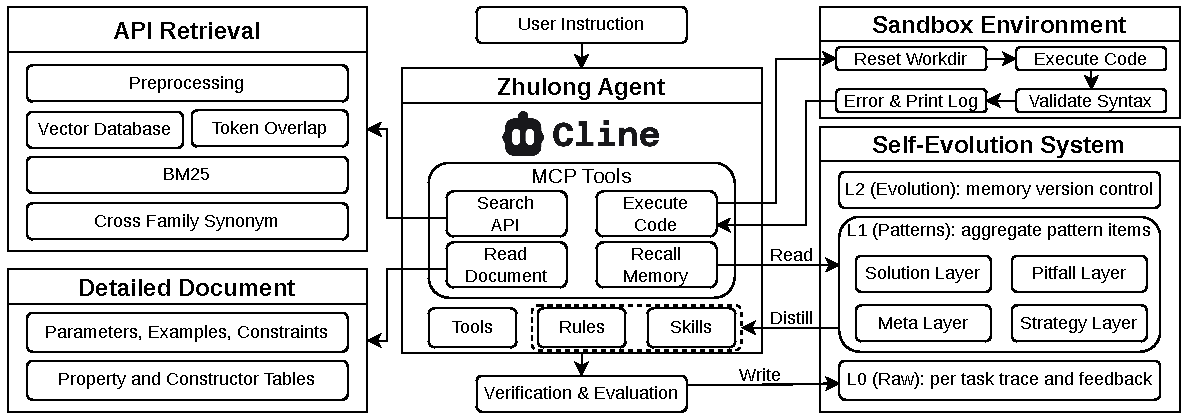
\includegraphics[width=0.85\linewidth]{figures/zhulong.pdf}
        \end{center}
    \end{figure}
    \vfill
    \begin{itemize}
        \item \textbf{Harness} (center): MCP tools --- API retrieval, documentation, sandbox execution, static checker
        \item \textbf{Self-evolution} (bottom right): L0/L1/L2 three-tier memory. Write side distills traces offline, read side re-injects knowledge at task time
    \end{itemize}
\end{frame}

\section{Harness}

\begin{frame}[fragile]{API Retrieval: Dual-Path with Heterogeneous Scores}
    \begin{itemize}
        \item \textbf{Semantic path}: embeds name + short summary, BM25 supplement
        \item \textbf{Keyword path}: camelCase split + \emph{bidirectional} abbreviation expansion
        \item Cross-family synonym map: \texttt{dbCrtRect} $\leftrightarrow$ \texttt{emyRect.create}
    \end{itemize}
    \vspace{4pt}
    \begin{exampleblock}{Query routing examples}
        \footnotesize
        \begin{tabular}{lll}
            \toprule
            Query & Type & What happens \\
            \midrule
            \texttt{"compress"} & full$\to$abbr & reverse-expand $\to$ \texttt{CP}, match APIs containing \texttt{CP} \\
            \texttt{"CV"} & abbr$\to$full & expand $\to$ CellView, match \texttt{dbOpenCV} \\
            \texttt{"dbCrtInst"} & fragment & exact-match hit $\to$ hint: read doc \\
            \texttt{"create net"} & NL & keyword + soft redirect to semantic \\
            \bottomrule
        \end{tabular}
    \end{exampleblock}
\end{frame}

\begin{frame}{Sandbox Execution \& Static Checker}
    \begin{itemize}
        \item \textbf{Multi-port isolation}: 4 independent sandbox endpoints, each with its own workdir $\to$ no state pollution, no pass-rate jitter
        \item \textbf{Static checker} (post-execution, non-blocking): rules derived from API docs + extensive testing, \textbf{no observed false positives}
    \end{itemize}
    \vspace{4pt}
    \begin{exampleblock}{Checker catches}
        \begin{itemize}
            \item Fabricated API --- calls a non-existent name
            \item Wrong keyword argument --- mismatched parameter name
            \item Native value for SWIG type --- e.g.\ plain \texttt{str} where \texttt{emyString} is required
            \item Failure ignorance --- \texttt{except} block that swallows an error
        \end{itemize}
    \end{exampleblock}
\end{frame}

\section{Self-Evolution}

\begin{frame}{Governed Self-Evolution: Write Side}
    \begin{block}{Principle: governance, not accumulation}
        Plausible-but-ungoverned experience can hurt~\cite{zhao2024expel,yang2026skillopt}. Every stage carries a reliability gate:
    \end{block}
    \begin{itemize}
        \item \textbf{Ground-truth anchoring}: override trace's self-report with evaluator verdict, force-fail when no verdict $\to$ no false-positive verified entries
        \item \textbf{Failure routing}: \\
        final self test errored $\to$ \emph{error path} \\
        self test passed but GT failed $\to$ \emph{contradiction path}
        \item \textbf{Scope boundary}: verified entries carry preconditions / constraints from trace facts only --- never inferred, never absolute ``avoid X''
        \item \textbf{Disconfirmation}: an entry failed on the same API twice is filtered before promotion
    \end{itemize}
\end{frame}

\begin{frame}{Governed Self-Evolution: Read Side}
    \begin{block}{Anti-leakage: structural, not gate-based}
        Under instance-disjoint splits, a held-out task could copy a sibling's verbatim answer. We prevent this structurally:
    \end{block}
    \begin{itemize}
        \item \textbf{Names-only pre-injection}: solution entries reduced to API names, dropping call sequence
        \item \textbf{Docstring generalization}: shared regex stripper on both distillation and query sides $\to$ same-family tasks match without verbatim leakage
        \item \textbf{Embed problem, return solution}: index matches on problem, agent receives the solution
        \item \textbf{Pitfalls not pre-injected}: routed to runtime query instead --- task description cannot predict which API will be misused
    \end{itemize}
    \vfill
    \footnotesize Held-out gate: a round is accepted only if validation pass rate does not regress by $>$5\%~\cite{yang2026skillopt}.
\end{frame}

\begin{frame}[fragile]{Distilled Knowledge: Two Examples}
    \begin{columns}
        \begin{column}{.48\textwidth}
            \begin{exampleblock}{Workflow skill:\\ \texttt{createlib}}
                \scriptsize
                Distilled from 5 passed tasks.\\[4pt]
                \textbf{Scenario}: create-instance-in-schematic-cellview\\
                \textbf{APIs}: \texttt{dbCreateLib}, \texttt{dbNewCV}, \texttt{dbOpenCVByType}, \texttt{dbCrtInst}, \texttt{emyPointF}\\[4pt]
                \textbf{Rule}: Initialize \texttt{emyInitAether} only if no existing session --- \emph{skip when the function receives an already-initialized \texttt{lib\_name}}
            \end{exampleblock}
        \end{column}
        \begin{column}{.48\textwidth}
            \begin{exampleblock}{Pitfall skill: \texttt{bbox-origin-shift}}
                \scriptsize
                Distilled from contradiction analysis.\\[4pt]
                \textbf{Finding}: spec says shift to bbox LB, but \texttt{print\_log} shows \texttt{cv.bbox: (0,0,0,0)} --- empty design, zero-area bbox\\[4pt]
                \textbf{Root cause}: code iterates \texttt{cv.shapes} on empty design, finds nothing, falls through to else branch with \texttt{(0,0)}\\[4pt]
                \textbf{Coverage gap}: \texttt{aeShiftOrigin} never reached
            \end{exampleblock}
        \end{column}
    \end{columns}
    \vfill
\end{frame}

\section{Experiments}

\begin{frame}{Harness Evaluation on 158 Tasks}
    \begin{columns}
        \begin{column}{.45\textwidth}
            \begin{table}[h]
                \centering
                \caption{Retrieval--experience decomposition}
                \scriptsize
                \begin{tabular}{llc}
                    \toprule
                    Experience & Retrieval & Pass@1 \\
                    \midrule
                    bare & semantic-only & 87.3\% \\
                    bare & full & 88.6\% \\
                    human & semantic-only & 89.9\% \\
                    human & full & \textbf{92.4\%} \\
                    \bottomrule
                \end{tabular}
            \end{table}
            \footnotesize Both retrieval and experience help.
        \end{column}
        \begin{column}{.45\textwidth}
            \begin{table}[h]
                \centering
                \caption{Cross-model transfer (158 tasks)}
                \scriptsize
                \begin{tabular}{lc}
                    \toprule
                    Model & Pass@1 \\
                    \midrule
                    DeepSeek-V4-Pro & \textbf{92.4\%} \\
                    GLM-5.2 & 91.1\% \\
                    Kimi-K2.6 & 89.2\% \\
                    DeepSeek-V4-Flash & 85.4\% \\
                    Doubao-Seed-2.0 & 71.5\% \\
                    \bottomrule
                \end{tabular}
            \end{table}
            \footnotesize Transfers across backbones down to a capability floor.
        \end{column}
    \end{columns}
\end{frame}

\begin{frame}{Failure Analysis}
    % \begin{columns}
        % \begin{column}{.55\textwidth}
            \begin{figure}[htpb]
                \begin{center}
                    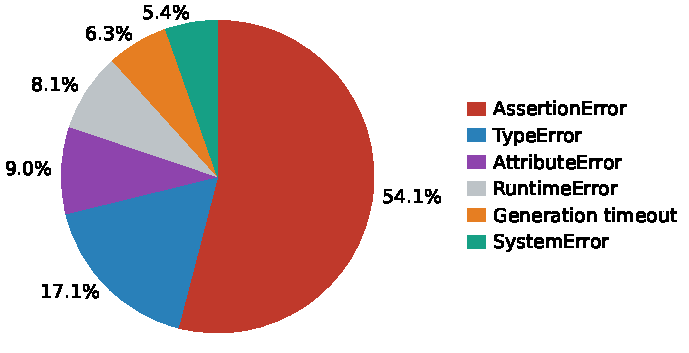
\includegraphics[width=0.8\linewidth]{figures/failure_type_distribution.pdf}
                \end{center}
            \end{figure}
        % \end{column}
        % \begin{column}{.4\textwidth}
            \footnotesize
            Aggregating 111 failures across 5 backbones:
            \begin{itemize}
                \item \textbf{AssertionError} dominates (54\%): code runs, but hidden test fails --- a \emph{logic} error, not syntax or type
                \item The static checker intercepts deterministic misuse (\texttt{TypeError}/\texttt{AttributeError})
                \item Majority of failures are \emph{semantic} $\to$ require real execution to expose
            \end{itemize}
        % \end{column}
    % \end{columns}
\end{frame}

\begin{frame}{Self-Evolution on Challenge Test}
    \begin{table}[h]
        \centering
        \caption{Evolution across rounds}
        \footnotesize
        \begin{tabular}{lcccc}
            \toprule
            Knowledge & Patterns & Skills & Pass@1 (test) & Pass@1 (val) \\
            \midrule
            bare & 0 & 0 & 66.0\%$\pm$7.2 & --- \\
            self-evolved R1 & 256 & 16 & 78.0\%$\pm$9.9 & 81.0\%$\pm$8.2 (accept) \\
            self-evolved R2 & 334 & 20 & \textbf{80.0\%}$\pm$3.1 & 88.0\%$\pm$2.7 (accept) \\
            self-evolved R3 & 386 & 25 & 75.5\%$\pm$6.7 & 80.0\%$\pm$3.5 (reject) \\
            \midrule
            human baseline & --- & 4 & 77.5\%$\pm$5.3 & --- \\
            \bottomrule
        \end{tabular}
    \end{table}
    \vspace{4pt}
    \begin{itemize}
        \item Self-evolution from bare start surpasses human baseline
        \item R2 peaks on both val and test, R3 regresses on both $\to$ gate correct
        \item Held-out gate rejects R3 $\to$ knowledge frozen at R2
    \end{itemize}
\end{frame}

\begin{frame}{Ablations: Write-Side Gates \& Read-Side Injection}
    \begin{columns}
        \begin{column}{.48\textwidth}
            \begin{table}[h]
                \centering
                \caption{Write-side gate ablation}
                \tiny
                \begin{tabular}{lccl}
                    \toprule
                    Gate & ON & OFF & Finding \\
                    \midrule
                    GT anchor & 37 & 48 & 12 false-pos. \\
                    contrad. & 37 & 54 & 17 more, low-prec. \\
                    routing & 36 & 37 & forced success, 0 pitfall \\
                    scope & 36 & 36 & not triggered \\
                    disconfirm & 37 & 37 & not triggered \\
                    \bottomrule
                \end{tabular}
            \end{table}
            \scriptsize GT anchoring strongest: prevents 50\% false-positive verified.
        \end{column}
        \begin{column}{.48\textwidth}
            \begin{table}[h]
                \centering
                \caption{Read-side ablation (val, 5 runs)}
                \scriptsize
                \begin{tabular}{lc}
                    \toprule
                    Configuration & $\Delta$ vs.\ baseline \\
                    \midrule
                    pitfall pre-inject on & $-$8.3 pp \\
                    generalization off & $-$6.6 pp \\
                    full-sequence inject & $-$5.0 pp \\
                    embed solution & 0 pp \\
                    \bottomrule
                \end{tabular}
            \end{table}
            \scriptsize Pitfall pre-injection most harmful. 3 of 4 mechanisms validated.
        \end{column}
    \end{columns}
\end{frame}

\section{Conclusion}

\begin{frame}{Conclusion}
    \begin{itemize}
        \item \textbf{Harness}: frozen-agent EDA scripting with retrieval, sandbox, and a static checker with no observed false positives $\to$ \textbf{92.4\%} on 158 tasks, transfers across 5 LLMs
        \item \textbf{Self-evolution}: governed three-tier memory with reliability gates and structural anti-leakage $\to$ from bare start, surpasses hand-written baseline (\textbf{80.0\%} vs.\ 77.5\%) on a harder challenge test
        \item \textbf{Ablations}: GT anchoring prevents 50\% false-positive knowledge. 3 of 4 read-side mechanisms validated
    \end{itemize}
    \vfill
    \begin{block}{Limitations \& Future Work}
        \footnotesize
        Small challenge test (40 tasks). Two write-side gates not triggered on the failure pool. Single EDA domain. Future: more tool flows, larger task sets, cross-domain governance.
    \end{block}
\end{frame}

\begin{frame}[allowframebreaks]
    \bibliographystyle{IEEEtran}
    \bibliography{reference}
\end{frame}

\begin{frame}
    \begin{center}
        {\Huge Thanks!}\\[12pt]
        {\large Questions?}
    \end{center}
\end{frame}

\end{document}
